% Klassifiziert den Dokumenten-Typ
% Doku: http://exp1.fkp.physik.tu-darmstadt.de/tuddesign/
% Farben: http://www.tu-darmstadt.de/media/medien_stabsstelle_km/services/medien_cd/das_bild_der_tu_darmstadt.pdf
%  bigchapter: Chapter haben doppelte Schriftgröße
%  linedtoc: Linien im Inhaltsverzeichnis wie bei Überschriften
%  colorbacktitle: Der Dokumenten-Titel wird mir der Accentfarbe hinterlegt
\documentclass[bigchapter,colorback,accentcolor=tud4b,linedtoc,11pt]{tudreport}

% Input Dokument hat das Encoding UTF-8
\usepackage[utf8]{inputenc}
% Wichtiges Paket für Links und verlinktes Inhaltsverzeichnis
\usepackage[ngerman]{hyperref}
% Paket für Fußnoten
\usepackage[stable]{footmisc}
\usepackage{multirow}
\usepackage{colortbl}
% Alternatives package für bilder
\usepackage{wrapfig}
% Paket für amsmath (aligned mathe formeln)
\usepackage{amsmath}
% "definiert als" usw.
\usepackage{mathtools}
% Farbige tabellen
\usepackage{colortbl}
 
% Paket für Bibliotheks-Verzeichnis, square: Verwende eckige statt runde klammern
% \usepackage[square]{natbib}
% Paket zum Plotten von Datensätzen
\usepackage{pgfplots}
\pgfkeys{%
  /pgfplots/default/.style={%
    /pgf/number format/use comma,
    legend pos=north west,
    width=0.9\linewidth,
    height=0.7\linewidth,
    scale only axis,
    xmin=0,
    ymin=0,
    grid=both,
    tick align=outside,
    tickpos=left,
    minor x tick num=3,
    minor y tick num=3,
    minor grid style={dotted,thin},
  }
}

% Anhänge für Original-Messdaten
\usepackage{fancyvrb}

% Verwende deutsche Bezeichner für Inhaltsverzeichnis, ... (ngerman = New German: neue Rechtschreibung)
\usepackage{ngerman}
% Deutsche Zahlen (entfernt z.B. das Leerzeichen nach einem Dezimal-Komma)
\usepackage{ziffer} 

\usepackage[verbose]{placeins}

%wegen Grafikverschiebung hinzugefügt
\usepackage{float}

%\usepackage{graphicx}
%\usepackage{caption}
\usepackage{subcaption} %Für subfigures

% PDF-Optionen
\hypersetup{%
  pdftitle={TU Darmstadt \- Physikalisches Praktikum für Fortgeschrittene},
  pdfauthor={Esra Bauer, Sören Link},
  pdfsubject={Versuch 4.11},
  pdfview=FitH,
}
% Nummeriere formeln in Subsections einzeln
% Kleines makro zur assymetrischen Fehlerangabe

% Entspricht-Zeichen
\usepackage{scalerel}

\newcommand\equalhat{%
\let\savearraystretch\arraystretch
\renewcommand\arraystretch{0.3}
\begin{array}{c}
\stretchto{
    \scalerel*[\widthof{=}]{\wedge}
    {\rule{1ex}{3ex}}%
}{0.5ex}\\ 
=%
\end{array}
\let\arraystretch\savearraystretch
}
%BEGINN TITELSEITE

\title{Optisches Pumpen}

\subtitle{Esra Bauer  \\Sören Link}

\subsubtitle{Tutor: Simon Mieth \hfill 29.6.2015}

\author{Esra Bauer, Sören Link}

%\settitlepicture{img/title.jpg}

\institution{Physikalisches Praktikum \\für Fortgeschrittene \\ Versuch 4.11}

\date{\today}
%ENDE TITELSEITE


\begin{document}
%ANFANG DOKUMENT

%Titelseite einfügen
\maketitle

%Inhaltsverzeichnis einfügen
\tableofcontents

%ANFANG INHALT
\chapter{Einleitung}

In diesem Versuch geht es um optisches Pumpen, d.h. Erzeugung einer von der thermischen Besetzungsverteilung (Boltzmann-Verteilung) abweichenden Verteilung an Rubidiumatomen, womit man beispielsweise die sehr feine Zeeman-Aufspaltung der Hyperfeinstrukturniveaus spektroskopieren kann. Wir bestrahlen dazu Rubidiumdampf in einem Glaskolben mit einer Rubidiumlampe. Unter anderem wird auch der Kernspin von Rubidium $^{87}$Rb und $^{85}$Rb ermittelt.

\chapter{Grundlagen}

\section{Optisches Pumpen}

Wir können den Rubidiumdampf als kanonisches Ensemble betrachten, d.h. als System, welches an ein Wärmebad der Temperatur T gekoppelt ist. Die Besetzungsverteilung ist dann von T abhängig und durch die Boltzmann-Statistik gegeben. Für die Zahl $N_j$ der Teilchen, die den Zustand j besetzen, gilt demnach:
$$N_j = N_0 \cdot g_j \cdot e^{- \beta E_j},$$
wobei $\beta = \frac{1}{k_B T}$ die Energienormierung bezeichnet und $g_j$ den Entartungsgrad der Energie $E_j$, also die Anzahl der Zustände gleicher Energie $E_j$.

Optisches Pumpen heißt, eine von dieser Statistik abweichende Besetzungsverteilung zu erzeugen. Um dies zu veranschaulichen, betrachten wir ein Energiesystem, das aus drei Niveaus besteht. C sei das höchste Niveau, B das mittlere und A das untere. Von den beiden Grundniveaus A und B seien optischen Übergänge zu C möglich, nicht aber zwischen A und B. Zu Beginn sind nun A und B gleichbesetzt, der Polarisationsgrad ist also: $P \coloneqq \frac{N_B-N_A}{N_B+N_A} = \frac{N_B-N_A}{N} = 0$.

\begin{figure}[H] 
  \centering
     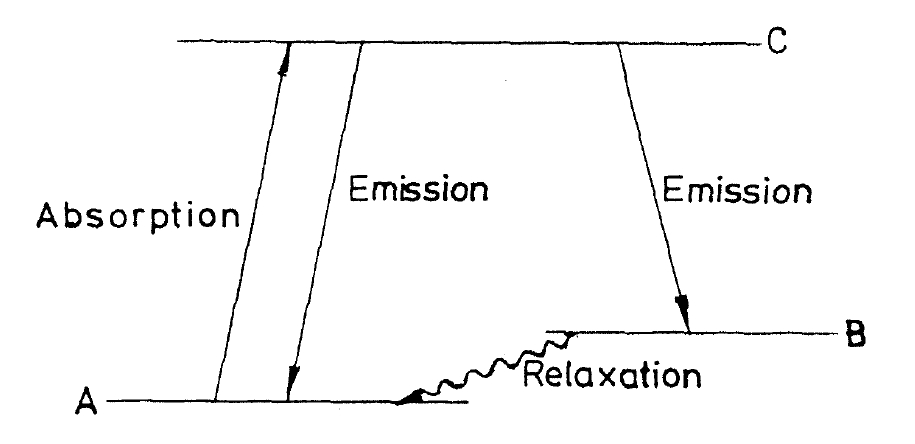
\includegraphics[width=0.5\textwidth]{img/Pumpen.jpg}
     \caption{Prinzip des optisches Pumpens am 3-Niveau-System.}
\end{figure}

Nun wird derartiges Licht eingestrahlt, dass nur der Übergang von A nach C induziert wird, von C können Übergänge nach A oder B stattfinden, jedoch nicht von B nach C. Dies bedeutet, immer mehr Teilchen besetzen das Niveau B und immer weniger das Niveau A, da sie von dort kontunierlich nach C gepumpt werden. Dem entgegen wirkt die sogenannte Relaxation, d.h. der Übergang von B nach A. Hier sind zwar keine optischen Übergange möglich, jedoch können Teilchen durch magnetische Dipolübergänge oder durch Stöße dennoch von B nach A übergehen. Man definiert daher die Relaxationsrate wie folgt: 
$$\frac{d n}{d t} \propto \frac{n}{T_1},~ n \coloneqq N_B-N_A$$
mit der Relaxationszeit $T_1$. Es lässt sich sinnvollerweise auch eine Pumpzeit finden. Diese ist abhängig von der Intensität und von $N_A$. Für die Zunahme der Besetzung $N_B$ von B gilt:
$$d N_B = - d N_A = -K \cdot I \cdot N_A \cdot d t,$$
wobei K eine Proportionalitätskonstante ist. Daraus ergibt sich:
$$d n = d (N_B-N_A) \propto -K \cdot I \cdot (N-n) \cdot d t,~ N_A = \frac{1}{2} (N-n).$$ 
Die Pumpzeit ist damit $T_P = \frac{1}{K \cdot I}$ und $\frac{d n}{d t} \propto \frac{N-n}{T_P}$.

Pumpen und Relaxation erfolgt gleichzeit, wir finden also folgende Differentialgleichung:
$$\frac{d n}{d t} = \frac{N-n}{T_P} - \frac{n}{T_1}$$
und nach kurzer Zeit stellt sich ein Gleichgewicht ein, so dass gelten muss $\frac{d n}{d t} = 0$, woraus folgt: $n_0 = \frac{N}{1+\frac{T_P}{T_1}}$. Um die DGL zu lösen, setze $\frac{1}{\tau} = \frac{1}{T_P} + \frac{1}{T_1}$. Man erhält folgende Lösungen für $n$ und $N_A$:
$$n = n_0 (1-e^{-\frac{t}{\tau}}),~~~ N_A = \frac{1}{2} (N-n_0 (1-e^{\frac{t}{\tau}})).$$

Beim Rubidiumdampf lässt sich der Erfolg des optischen Pumpens (d.h. der Pumpvorgang muss gegenüber der Relaxation überwiegen) an der Transparenz erkennen. Da das Pumplicht nur den Übergang von A nach C induziert, wird dieses Licht zu Anfang stark absorbiert, da noch viele Teilchen im Niveau A befindlich sind und beim Übergang nach C jeweils Licht absorbieren. Je weniger Teilchen sich in A aufhalten, d.h. je stärker der Pumpvorgang fortschreitet, desto weniger Licht wird also absorbiert, wodurch die Transparenz des Rubidiumdampfes sinkt. 

\section{Energieniveaustruktur von Rubidium}

Das Rubidium-Atom besitzt ein s-Valenzelektron, d.h. der Grundzustand ist ein $^2S_{\frac{1}{2}}$-Zustand. Der Spin hat also die Quantenzahl $S = \frac{1}{2}$, der Bahndrehimpuls die Quantenzahl $L = 0$ und der Gesamtdrehimpuls $J = L + S = \frac{1}{2}$. Die Feinstrukturaufspaltung, die im Wesentlichen auf der L-S-Kopplung beruht, geschieht also erst ab dem ersten angeregten Zustand mit $L = 1$; der Gesamtdrehimpuls kann nun die Werte $\frac{1}{2}$ und $\frac{3}{2}$ annehmen. Zusätzlich gibt es die Hyperfeinstruktur, die eine Entartung aufgrund der verschiedenen Kopplungsmöglichkeiten des Kernspins $I$ und des Hüllendrehimpulses $J$ bezeichnet. Der Gesamtdrehimpuls $F = I + J$ kann alle ganzzahligen Werte zwischen $|J-I|$ und $|J+I|$ annehmen. Auf die resultierenden Hyperfeinstrukturniveaus wirkt der Zeeman-Effekt, falls ein äußeres Magnetfeld angelegt wird, entarten diese Niveaus also je nach Raumrichtung des Gesamtdrehimpulses und es gibt zusätzlich $2F$ Zeeman-Niveaus mit $m_F = -F, -F+1, ..., +F$. Folgende Termschemata zeigen dies in übersichtlicher Weise:

\begin{figure}[H]
\begin{subfigure}[c]{0.52\textwidth}

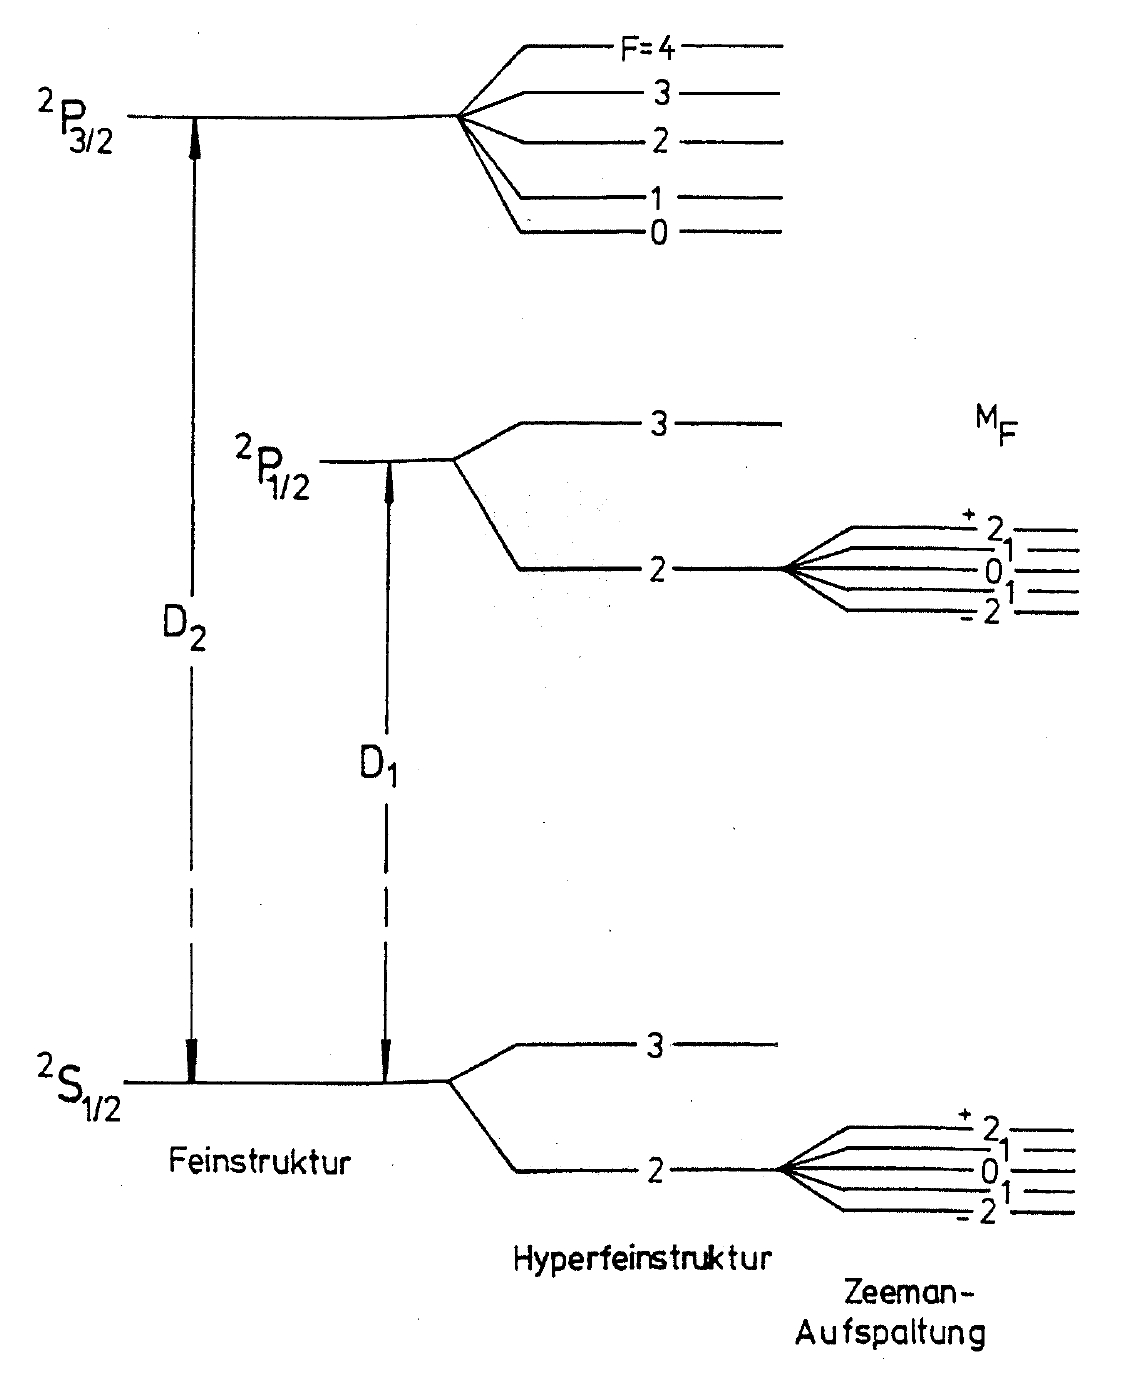
\includegraphics[width=0.9\textwidth]{img/Rb-85.jpg}
\subcaption{Termschema von $^{85}$Rb.}

\end{subfigure}
\begin{subfigure}[c]{0.52\textwidth}
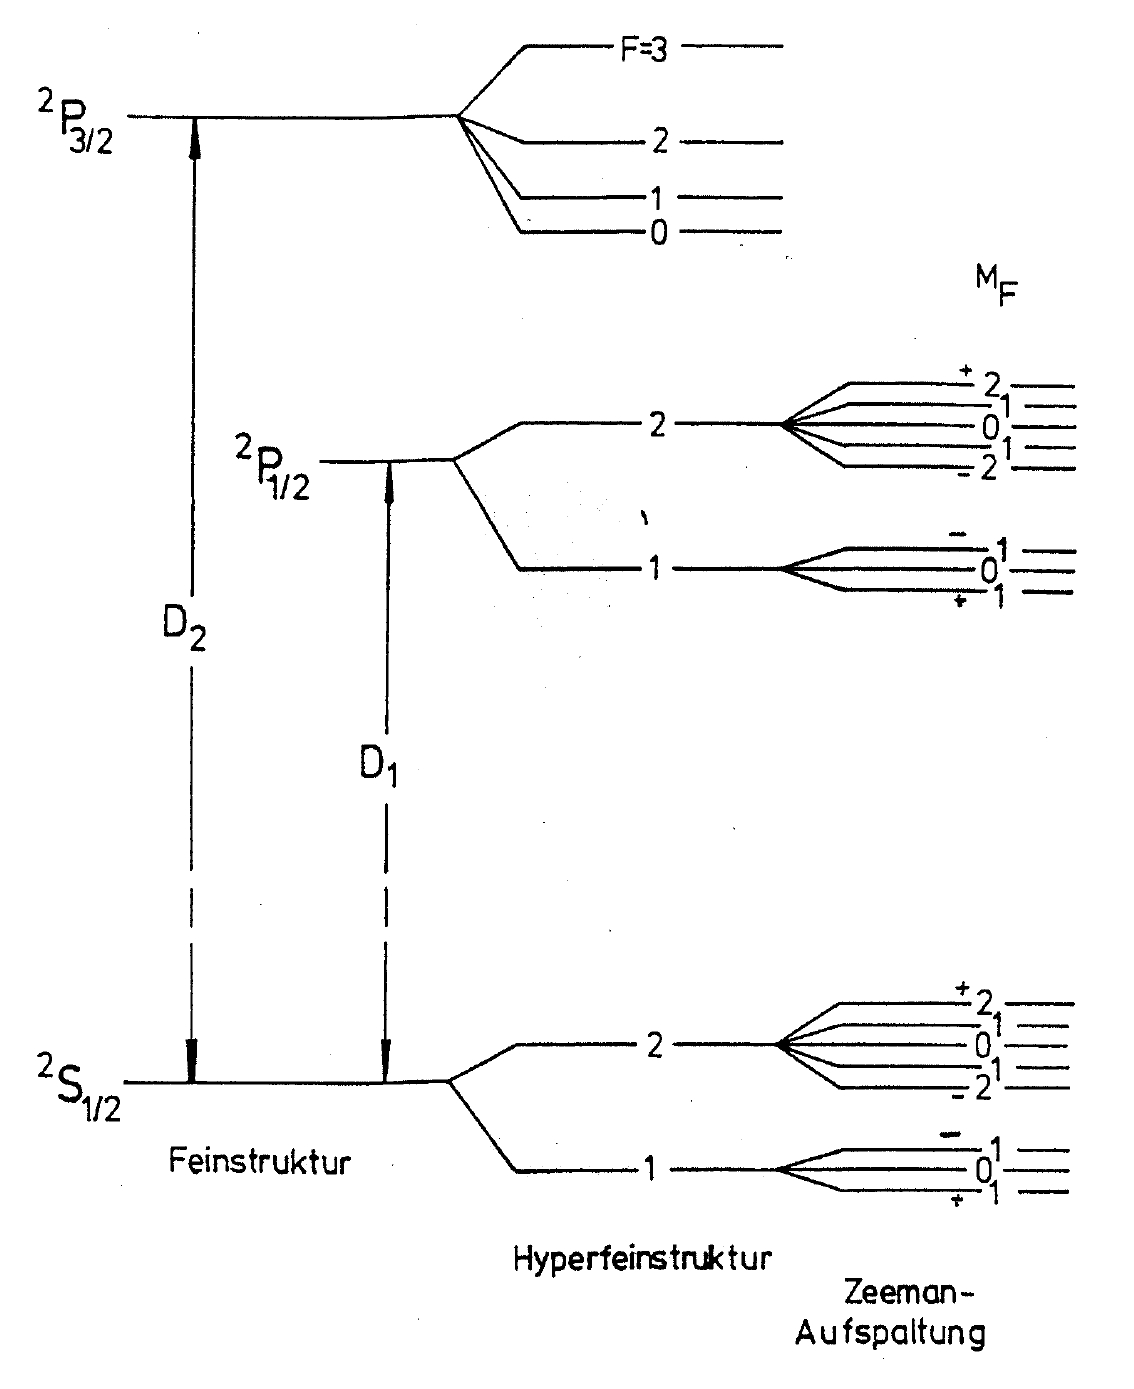
\includegraphics[width=0.9\textwidth]{img/Rb-87.jpg}
\subcaption{Termschema von $^{87}$Rb.}
\end{subfigure}
\caption{Termschemata der verwendeten Isotope.}
\end{figure}

Betreffend die Übergänge zwischen den Niveaus gibt es folgende Auswahlregeln für elektronische Dipolübergänge (optische Übergänge): $\Delta J = 0, \pm 1,~ 0 \nleftrightarrow 0$, 
$\Delta M_J = 0, \pm 1$ ($ 0\nleftrightarrow 0 $, falls $\Delta J = 0$),
$\Delta L = \pm 1$.
Das heißt, es sind keine elektronischen Dipolübergänge zwischen den Zeeman- und den Hyperfeinstrukturniveaus eines Feinstrukturniveaus möglich. Möglich sind hier jedoch magnetische Dipolübergänge, denn für diese gilt für die Bahndrehimpulsquantenzahl die Auswahlregel $\Delta L = 0$. Die übrigen Auswahlregeln gelten wie oben.

Die Energien der Zeeman-Niveaus lassen sich mittels der Breit-Rabi-Formel berechnen, die für $J = \frac{1}{2}$ gilt und den Vorteil besitzt, dass sie sowohl für schwache Magnetfelder gültig ist, also für reinen Zeeman-Effekt, als auch für den Übergangsbereich zu starken Magnetfeldern (dann tritt der Paschen-Back-Effekt auf). Sei $\Delta E$ der Energieabstand der Hyperfeinstrukturniveaus, $g_I$ der g-Faktor des Kerns in Einheiten des Bohrschen Magnetons, $g_J$ der g-Faktor der Elektronenhülle, $\mu_B$ das Bohrsche Magneton und $B$ die magnetische Flussdichte, dann ist die Energie der Zeeman-Niveaus für $F = I \pm J$ gegeben durch:
$$E(F,m_F) = - \frac{\Delta E}{2 (2I + 1)} + \mu_B g_I B m_F \pm \frac{\Delta E}{2} ( 1 + \frac{4 m_F}{2I+1} \xi + \xi^2 )^{\frac{1}{2}}$$
mit $\xi = \frac{\mu_B (g_J - g_I)}{\Delta E} B.$

\section{Spektroskopie der Zeeman-Niveaus nach optischem Pumpen}

Pumpt man nun mit zirkular polarisiertem Licht, lassen sich Übergänge zwischen den Zeeman-Niveaus induzieren. Bei Bestrahlung mit $\sigma^+$-Pumplicht werden Übergänge innerhalb eines Hyperfeinstrukturniveaus von den negativen magnetischen Quantenzahlen $m_F$ zu den positiven induziert und bei Bestrahlung mit $\sigma^-$-Pumplicht reichern sich entsprechend die Zeeman-Niveaus mit negativen $mF$ an. Ändert man die Polarisation von $\sigma^+$ nach $\sigma^-$, werden Übergänge zwischen den Zeeman-Niveaus mit $\Delta m_F = -1$ ermöglicht, während sich die Transparenz des Rubidiumdampfes in Folge der Umbesetzung verändert.

Im Gegensatz zur Bestrahlung mit $\sigma^-$-Pumplicht bewirkt die Einstrahlung eines linear polarisieren, magnetischen Wechselfeldes der richtigen Frequenz vermehrt Übergänge vom jeweils höheren Zeeman-Niveau zum nächst niederen Niveau. Die Frequenz dieser Übergänge ist nach Breit-Rabi: 

$$f(m_F \leftrightarrow m_F-1) = \pm \frac{\mu_B g_I B}{h} + \frac{\Delta E}{2h} \left( ( 1 + \frac{4 m_F}{2I+1} \xi + \xi^2 )^{\frac{1}{2}} - ( 1 + \frac{4 (m_F - 1)}{2I+1} \xi + \xi^2 )^{\frac{1}{2}} \right).$$

\section{Bestimmung des Kernspins}

Das Prinzip der Bestimmung des Kernspins ist folgendes: Mit einem magnetischen Hochfrequenzfeld werden magnetische Dipolübergänge zwischen benachbarten Zeeman-Niveaus im Grundzustand der Rubidium-Atome induziert und aus der so bestimmten Zeeman-Aufspaltung wird auf die Kernspins der beiden Isotope geschlossen. Im Resonanzfall gilt gerade $\Delta E = h \nu$ und da wir für die Zeeman-Energien bereits Formeln kennengelernt haben, die eine Abhängigkeit vom Kernspin und von der magnetischen Flussdichte aufweisen, müssen wir bei gegebener Frequenz des Magnetfeldes und gegebener Flussdichte lediglich noch nach $I$ umstellen. Ob Resonanz vorliegt, lässt sich wiederum über die Transparenz des Rubidiumdampfes feststellen. Durch Bestrahlung mit zirkular polarisiertem ($\sigma^-$-) Licht findet optisches Pumpen statt, d.h. die Zelle mit Rubidiumdampf wird transparent. Erfüllt das Magnetfeld, dessen Wirkung dem optischen Pumpen entgegengerichtet ist, nun die Resonanzbedingung, wird folglich die Zelle wieder weniger transparent. D.h. man kann nun entweder $B$ festhalten und die Frequenz variieren oder wahlweise die Frequenz festhalten und $B$ variieren, bis die Resonanzbedingung erfüllt ist. Relevant ist für die Berechnung noch die magnetische Flussdichte im Zentrum eines Helmholtz-Spulenpaares (Radius $R$, Windungszahl $N$) in Abhängigkeit des Spulenstroms $I$:
$$B_Z = \frac{\mu_0 n \cdot I}{{\left( \frac{5}{4}\right)}^{1,5} R}$$
mit der Vakuumpermeabilität $\mu_0 \coloneqq 4\,\pi \cdot 10^{-7} \frac{\mathrm{N}}{\mathrm{A}^2} = 12{,}566\,370\,614\ldots \cdot 10^{-7} \frac{\mathrm{N}}{\mathrm{A}^2}$.

Ebenfalls sollte Erwähnung finden, dass sich der Kernspin auch durch simples Abzählen der Zeeman-Niveaus ermitteln lässt, da bekanntermaßen die Zahl der Zeeman-Niveaus $2F$ beträgt und $F= I+J$, wobei $J$ bekannt ist.

\chapter{Aufbau und Durchführung}

Der Aufbau besteht im Wesentlichen aus der Absorptionskammer, welche mit Rubidium gefüllt ist, der Pumplichtquelle (Rubidium-Gasentladungslampe) sowie der Helmholtz-Spulenpaare für die Zeeman-Aufspaltung und zwei weitererer Spulen für das HF-Feld. Durch Vorwärmung mittels eines Kühlmittelumlaufsystems mit Thermostat wird die Temperatur der Absorptionskammer auf 55 $^{\circ}$C gehalten, wodurch das Rubidium verdampft. Desweiteren sind optische Komponenten für die Bereitstellung eines fokussierten zirkular polarisierten Lichtstrahls vonnöten. Die Intensität des transmittierten Lichtes wird mittels eines Silizium-Photodetektors gemessen. Im Folgenden ist der Aufbau schematisch dargestellt:

\begin{figure}[H] 
  \centering
     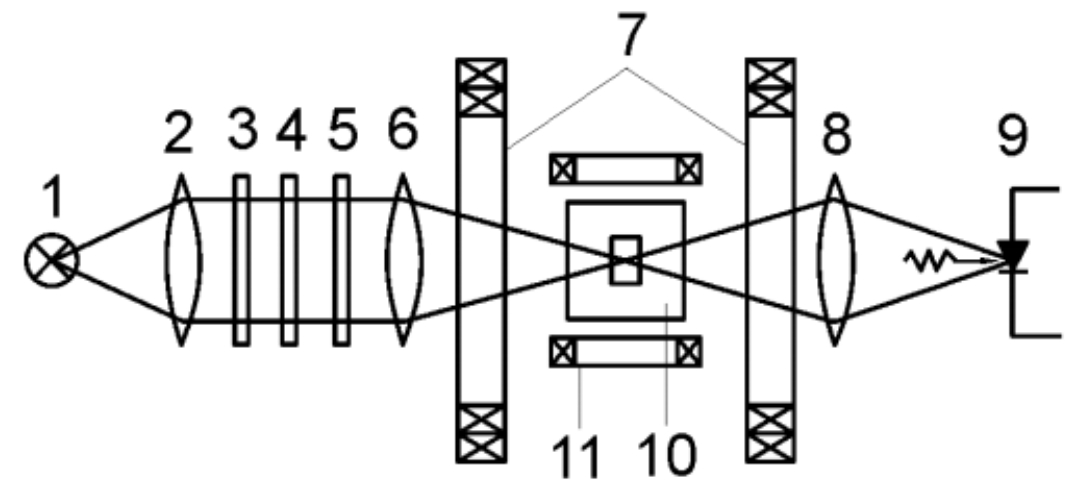
\includegraphics[width=0.5\textwidth]{img/Aufbau.jpg}
     \caption{Schematische Zeichnung des Versuchaufbaus \cite{Anleitung}.}
\end{figure}

Dabei bezeichnet

1 die Pumplichtquelle,

2, 6 und 8 Linsen zur Strahlformung,

3 einen Farbfilter,

4 einen linearen Polarisationsfilter,

5 ein $\frac{\lambda}{4}$-Plättchen,

7 die Helmholtz-Spulen für die Zeeman-Aufspaltung,

9 den Photodetektor,

10 die Absorptionskammer und

11 die HF-Spulen.

\chapter{Auswertung}

\section{Bestimmung der Pump- und Relaxationszeiten}
\begin{figure}[h]
\begin{tikzpicture}
  \begin{axis}[
    default,
    title={Intensität des Pumplichts, ohne Graufilter},
    legend pos=south east,
    xlabel=t in s,
    ylabel=U in V,
    xmin=0,
    xmax=0.24,
    ymin=-0.14,
    ymax=-0.02,
    yticklabel style={/pgf/number format/fixed},
    xticklabel style={/pgf/number format/fixed},
    width=0.4\textwidth,
    height=0.4\textwidth
  ]
  \addplot[black, only marks,mark=+, mark size=1pt] table[x index=0, y index=1] 
  {data/processed/NoFilter-afterCut.txt};
  \addlegendentry{Experimentelle Werte}

  \addplot[white!60!black, only marks,mark=+, mark size=1pt] table[x index=0, y index=1] 
  {data/processed/NoFilter-beforeCut.txt};
  \addlegendentry{für Fit verwendete Werte}

  \addplot[red, mark=x, mark size=0pt, samples=40, domain=0:0.24, thick]
  {0.5*(-0.3511274620028062 + 0.2858601201009212*(1 - exp(-33.74639279261045*x)))};
  \addlegendentry{Fit-Gerade}
\end{axis}
\end{tikzpicture}
%
\begin{tikzpicture}
  \begin{axis}[
    default,
    title={Intensität des Pumplichts, mit Graufilter},
    legend pos=south east,
    xlabel=t in s,
    ylabel=U in V,
    xmin=0,
    xmax=0.24,
    ymin=0.235,
    ymax=0.27,
    yticklabel style={/pgf/number format/fixed},
    xticklabel style={/pgf/number format/fixed},
    width=0.4\textwidth,
    height=0.4\textwidth
  ]

  \addplot[black, only marks,mark=+, mark size=1pt] table[x index=0, y index=1] 
  {data/processed/WithFilter-afterCut.txt};
  \addlegendentry{Experimentelle Werte}

  \addplot[white!60!black, only marks,mark=+, mark size=1pt] table[x index=0, y index=1] 
  {data/processed/WithFilter-beforeCut.txt};
  \addlegendentry{für Fit verwendete Werte}

  \addplot[red, mark=x, mark size=0pt, samples=40, domain=0:0.24, thick]
  {0.5*(0.47299234320540423 + 0.055588524545789504*(1 - exp(-27.016294865042738*x)))};
  \addlegendentry{Fit-Gerade}
\end{axis}
\end{tikzpicture}
\captionof{figure}{Gemessene Intensität des Lichts nach Durchlaufen des
  Rubidiums direkt nach Umpolung des Magnetfeldes. Da die Transparenz von
  Rubidium für das Pumplicht sich während des Pumpvorganges ändert, ist diese
  Proportional zur Besetzungszahl $N_A$. Insgesamt wurden zusammen 10 Messungen
  für die Einstellung mit und ohne Graufilter aufgenommen.}
\end{figure}


\section{Bestimmung des Kernspins von $^{87}Rb$ und $^{85}Rb$}
\begin{figure}[H]
    \centering
    \begin{subfigure}[H]{0.44\textwidth}
        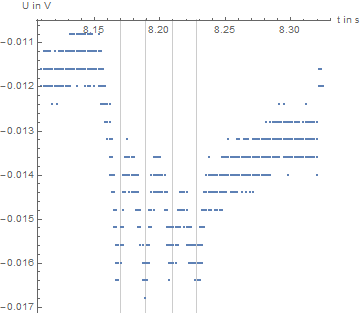
\includegraphics[width=1\textwidth]{img/2-1-plot1.png}
    \end{subfigure}%
    \qquad
    ~%add desired spacing between images, e. g. ~, \quad, \qquad, \hfill etc.
        %(or a blank line to force the subfigure onto a new line)
    \begin{subfigure}[H]{0.44\textwidth}
        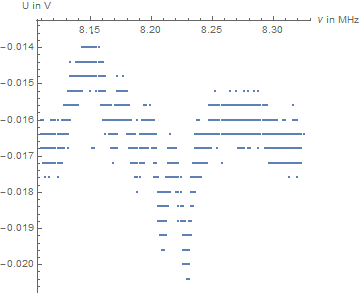
\includegraphics[width=1\textwidth]{img/2-1-plot2.png}
    \end{subfigure}
    \captionof{figure}{Absorptionspeaks von $^{85}Rb$ für $\sigma+$ und
      $\sigma-$ Pumplicht in Abhängigkeit der Frequenz des angelegten
      Magnetfeldes. Die senkrechten Linien markieren die Position der
      abgelesenen Werte. Insgesamt konnten wir 4 Absorptionspeaks
      identifizieren.}
\end{figure}


\begin{figure}[H]
    \centering
    \begin{subfigure}[H]{0.44\textwidth}
        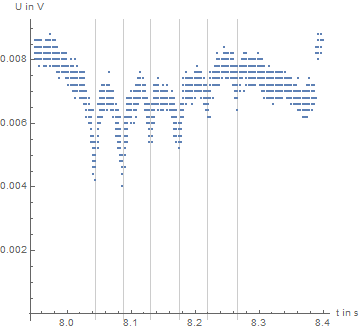
\includegraphics[width=1\textwidth]{img/2-1-plot3.png}
    \end{subfigure}%
    \qquad
    ~%add desired spacing between images, e. g. ~, \quad, \qquad, \hfill etc.
        %(or a blank line to force the subfigure onto a new line)
    \begin{subfigure}[H]{0.44\textwidth}
        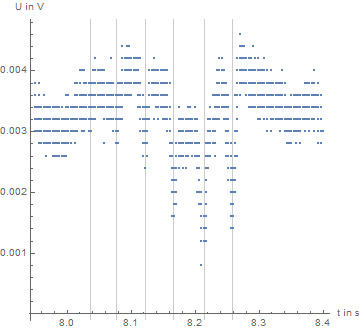
\includegraphics[width=1\textwidth]{img/2-1-plot4.png}
    \end{subfigure}
    \captionof{figure}{Absorptionspeaks von $^{87}Rb$ für $\sigma+$ und
      $\sigma-$ Pumplicht in Abhängigkeit der Frequenz des angelegten
      Magnetfeldes. Die senkrechten Linien markieren die Position der
      abgelesenen Werte. Insgesamt konnten wir 6 Absorptionspeaks
      identifizieren.}
\end{figure}


\chapter{Fazit}

%ENDE INHALT
\cleardoublepage{}
% Eintrag fürs Inhaltsverzeichnis
\newpage
\begin{thebibliography}{100}
  \bibitem{Anleitung} {Anleitung zum Versuch, heruntergeladen am 15.07.2015 von der Homepage der TU-Darmstadt.} 
  \bibitem{na22decay} {Semibyte, homepage of physics lab assistent and qualified
      computer scientist Tobias Krähling:
      \url{http://www.semibyte.de/wp/download/graphicslib/physics/termschema_na22.png}
    [CC BY-NC-SA 3.0]}
  \bibitem{cs137decay} {Wikipedia, the free encyclopedia. By Tubas-en [Public
      domain], via Wikimedia Commons: \url{http://upload.wikimedia.org/wikipedia/commons/thumb/3/3e/Cs-137-decay.svg/500px-Cs-137-decay.svg.png}}
\end{thebibliography}
\end{document}

%%% Local Variables:
%%% mode: latex
%%% TeX-master: t
%%% End:
